\documentclass[journal,10pt,twocolumn]{article}
\usepackage{graphicx}
\usepackage[margin=0.5in]{geometry}
\usepackage{amsmath}
\usepackage{array}
\usepackage{booktabs}
\usepackage{listings}
\providecommand{\norm}[1]{\left\lVert#1\right\rVert}
\providecommand{\abs}[1]{\left\vert#1\right\vert}
\usepackage{enumerate}
\let\vec\mathbf
\newcommand{\myvec}[1]{\ensuremath{\begin{pmatrix}#1\end{pmatrix}}}
\newcommand{\mydet}[1]{\ensuremath{\begin{vmatrix}#1\end{vmatrix}}}
\providecommand{\brak}[1]{\ensuremath{\left(#1\right)}}
\lstset{
frame=single,
breaklines=true,
columns=fullflexible
}
\title{\textbf{Matrix conic Assignment}}
\author{Mukesh Guptha.CH}
\date{September 2022}
\begin{document}
\maketitle
\paragraph{\textit{Problem Statement} - The equation of the common tangent touching the circle $x^2$+$y^2$=2 and the parabola $y^2$=8x above the x-axis is: }

\section*{Solution}
\begin{figure}[h]
\centering
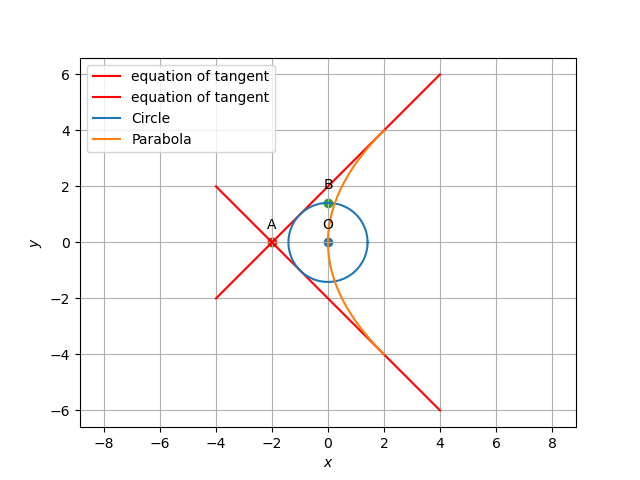
\includegraphics[width=1\columnwidth]{Figure.png}
\caption{Two tangent is drawn to the circle and parabola}
\label{fig:Curve}
\end{figure}
\section*{Solution}
\subsection*{Part 1}
\section*{Construction}
The input parameters are equation of the curve and the point of contacts \vspace{2mm}\\
{
\setlength\extrarowheight{2pt}
\begin{tabular}{|c|c|c|}
	\hline
	\textbf{Symbol}&\textbf{Value}&\textbf{Description}\\
	\hline
	\textbf{O}&$\begin{pmatrix}
	0\\
	0 \\
	\end{pmatrix}$&Centre of circle \\
	\hline
	r&$\sqrt{2}$&Radius of circle\\
	\hline
	\textbf{F}&$\begin{pmatrix}
	a\\
	0 \\
	\end{pmatrix}$&Focus of parabola\\
	\hline
	a&2&Given value of a\\
	\hline
	\textbf{q}&$\begin{pmatrix}
	x1 \\
	y1 \\
	\end{pmatrix}$&point of contact of parabola\\ 
	\hline
	\textbf{$q_1$}&$\begin{pmatrix}
	\frac{1.414}{\sqrt{16+y_1^2}}\\
    \frac{1.414}{\sqrt{4+y_1^2}} \\
	\end{pmatrix}$&point of contact of circle \\
	\hline
\end{tabular}
}
\subsection*{Part 2}
The standard equation of the parabola is given as :
\begin{align}
\vec{x}^{\top}\vec{V}\vec{x}+2\vec{u}^{\top}\vec{x}+f=0
\end{align}
The directrix of parabola is given as:
\begin{align}
		n_1^Tx=c	
\end{align}
where
\begin{align}
	\label{eq:V_matrix}
	\vec{X} &= \myvec{x \\
	                   y \\},
	\\
	\label{eq:u_vector}
	\vec{n_1} &= \myvec{a\\0},
	\\
	\label{eq:f_value}
	f &= 0
	%\\
	\\
	c&=-a
\end{align}
The equation of  a parabola with directrix $\vec{n}^{\top}\vec{x} = c$, eccentricity $e$ and focus $\vec{F}$ is given by 
\begin{align}
    \label{eq:conic_quad_form}
    \vec{x}^{\top}\vec{V}\vec{x}+2\vec{u}^{\top}\vec{x}+f=0
    \end{align}
where     
\begin{align}
  \label{eq:conic_quad_form_v}
\vec{V} &=\norm{\vec{n}}^2\vec{I}-e^2\vec{n}\vec{n}^{\top}, 
\\
\label{eq:conic_quad_form_u}
\vec{u} &= ce^2\vec{n}-\norm{\vec{n}}^2\vec{F}, 
\\
\label{eq:conic_quad_form_f}
f &= \norm{\vec{n}}^2\norm{\vec{F}}^2-c^2e^2
%\\
\\
e&=1
\\
\vec{V}&=\begin{pmatrix}
	0 & 0\\
	0 & 1\\
	\end{pmatrix} \\
    \vec{u}&=\begin{pmatrix}
	-4 \\
	0 \\
	\end{pmatrix} \\
	f&=0
    \end{align}
The equation of circle is given as :
\begin{align}
    \label{eq:conic_quad_form}
    \vec{x}^{\top}\vec{V_1}\vec{x}+2\vec{u_1}^{\top}\vec{x}+f_1=0
    \end{align}
where
\begin{align}
\vec{V_1}&=\begin{pmatrix}
	1 & 0\\
	0 & 1\\
	\end{pmatrix} \\
    \vec{u_1}&=\begin{pmatrix}
	0\\
	0 \\
	\end{pmatrix} \\
	f_1&=-2
    \end{align}
Consider the equation of parabola :
Given the point of contact $\vec{q}$, the equation of a tangent to  \\ $\vec{x}^{\top}\vec{V}\vec{x}+2\vec{u}^{\top}\vec{x}+f=0$ is 
  \begin{align}
  \brak{\vec{V}\vec{q}+\vec{u}}^{\top}\vec{x}+\vec{u}^{\top}\vec{q}+f = 0
  \label{eq:conic_tangent_final}
  \end{align}
where 
\begin{align}
\vec{V}&=\begin{pmatrix}
	0 & 0\\
	0 & 1\\
	\end{pmatrix} \\
    \vec{u}&=\begin{pmatrix}
	-4 \\
	0 \\
	\end{pmatrix} \\
	f&=0 \\
	\vec{X}&=\begin{pmatrix}
	x \\
	y \\
	\end{pmatrix} \\
\end{align}
By substituting the above values in tangent equation we get :
\begin{align}
\vec{-4x+yy_1-4x_1}=0
\end{align}
From the above equation the normal vector of tangent to the parabola is given by 
\begin{align}
\vec{n}&=\begin{pmatrix}
	-4 \\
	y1 \\
	\end{pmatrix}
\end{align}
Consider the equation of circle:
\begin{align}
\vec{x}^{\top}\vec{V_1}\vec{x}+2\vec{u_1}^{\top}\vec{x}+f_1=0
\end{align}
  If $\vec{V}^{-1}$ exists, given the normal vector $\vec{n}$, the tangent points of contact to circle  is given by
\begin{align}
  \begin{split}
\vec{q_1} &= \vec{V_1}^{-1}\brak{\kappa_i \vec{n}-\vec{u_1}}
\\
\text{where }\kappa &= \pm \sqrt{
\frac{
f_0
%\vec{u_1}^{\top}\vec{V_1}^{-1}\vec{u_1}-f_1
}
{
\vec{n}^{\top}\vec{V_1}^{-1}\vec{n}
}
}
  \end{split}
\label{eq:conic_tangent_qk}
\end{align}
\begin{align}
\kappa^2 \vec{n}^{\top}\vec{V_1}^{-1}\vec{n} - \vec{u_1}^{\top}\vec{V_1}^{-1}\vec{u_1} + f_1 =0 \\
\kappa = \pm \sqrt{
\frac{
\vec{u_1}^{\top}\vec{V_1}^{-1}\vec{u_1}-f_1
%\vec{u_1}^{\top}\vec{V_1}^{-1}\vec{u_1}-f_1
}
{
\vec{n}^{\top}\vec{V_1}^{-1}\vec{n}
}
}
\end{align}
By solving the above equation the point of contact of tangent to circle with normal vector $\vec{n}$ is given by :
\begin{align}
\vec{q_1} = 
\begin{pmatrix}
\frac{1.414}{\sqrt{16+y_1^2}} \\
\frac{1.414y1}{\sqrt{16+y_1^2}} 
\end{pmatrix}
\end{align}
The point of contact of tangent to parabola is :
\begin{align}
q&=
\begin{pmatrix}
\frac{y_1^2}{8} \\
 y_1 \\
\end{pmatrix}
\end{align}
The direction vector of tangent is given as :
\begin{align}
\vec{q}-\vec{q_1}
\end{align}
In order to get the value of y1 :
\begin{align}
\vec{n}^T(\vec{q}-\vec{q1})=0
\end{align}
By simplifying the above equation we will be geting the value of $y_1$:

\begin{enumerate}
\item The value of y1 is :
\begin{align}
y_1&=4
\end{align}
 \item The point of contact of tangent to parabola is :
\begin{align}
\vec{q}=
\begin{pmatrix}
2 \\
4 \\
\end{pmatrix}
\end{align}
\item The point of contact of tangent to circle is :
\begin{align}
\vec{q_1}=
\begin{pmatrix}
0.3516 \\
0.3516 \\
\end{pmatrix}
\end{align}
\item The normal vector of tangent is :
\begin{align}
\vec{n}=
\begin{pmatrix}
-4 \\
4 \\
\end{pmatrix}
\end{align}
\end{enumerate}
Hence the equation of common tangents to the circle and parabola is :
\begin{align}
\vec{n}^{T}(\vec{X}-\vec{q})=0
\end{align}
1st tangent is :
\begin{align}
\vec{x-y+2}=0
\end{align}
similarly 2nd tangent is: 
\begin{align}
\vec{x+y+2}=0
\end{align}
\end{document}
